\section{Mathematical and Numerical Models}\label{sec:MNmodels}

Assume we have a uniform mesh $x_1, x_2, \dots x_n$ with $\Delta x = x_{n+1} - x_n$ and that we know the values of a function $u$ at all the grid points, that is $u_i = u(x_i)$ for all $i$. We would like to find an approximation of the function $u(x)$ at the point $x^*$ other than the nodes $x_i$, with $x_{i-\frac{1}{2}} < x^* < x_{i+\frac{1}{2}}$, where $x_{i-\frac{1}{2}}$ and $x_{i+\frac{1}{2}}$ are the cell interfaces.

For a $r^{th}$ order accurate interpolation, there are $r$ candidate stencils next to the target point $x^*$: we denote these stencil as $S_k$, where $k=0, \dots, r-1$ labels the stencils from the leftmost stencil to the rightmost stencil in that order. Using  the Lagrange form of the interpolation polynomial, the polynom $p_k(x)$ over the stencil $S_k$ can be written as:

\begin{equation}
  \label{eq:Lagrange}
  p_k(x^*) = \sum_{j=0}^{r-1} u_{i-r+k+j+1} \sum_{\substack{l=0 \\ l \neq j}}^{r-1} \frac{x^* - x_{i-r+k+l+1}}{x_{i-r+k+j+1} - x_{i-r+k+l+1}} = \sum_{j=0}^{r-1} a_{k,i-r+j+1} u_{i-r+k+j+1}
\end{equation}

where $a_{k,i-r+j+1}$ are the Lagrange coefficients of the stencil $S_k$.

In table~\ref{tab:polynomial_coefficients} are reported the polynomial coefficients from $r=2$ to $r=9$ for all the interpolating stencils, for $x^* = x_{i+\frac{1}{2}}$; polynomial coefficients for $x^*=x_{i-\frac{1}{2}}$ can be obtained by table~\ref{tab:polynomial_coefficients} by symmetry.

\begin{table}
  \begin{center}
    \caption{Polynomial coefficients from $r=2$ to $r=9$ for $x^*=x_{i+\frac{1}{2}}$}
    \label{tab:polynomial_coefficients}
    \begin{tabular}{ccccccccccc}
      \toprule
      $r$  &  $k$  &  $j=0$  &  $j=1$  &  $j=2$  &  $j=3$  &  $j=4$  &  $j=5$  &  $j=6$  &  $j=7$  &  $j=8$  \\
      \midrule
      9  &  0  &  $ \frac{6435}{32768}$  &  $-\frac{7293}{4096}$  &  $ \frac{58905}{8192}$  &  $-\frac{69615}{4096}$  &  $ \frac{425425}{16384}$  &  $-\frac{109395}{4096}$  &  $ \frac{153153}{8192}$  &  $-\frac{36465}{4096}$  &  $ \frac{109395}{32768}$ \\ \addlinespace
         &  1  &  $-\frac{ 429}{32768}$  &  $ \frac{ 495}{4096}$  &  $-\frac{ 4095}{8192}$  &  $ \frac{ 5005}{4096}$  &  $-\frac{ 32175}{16384}$  &  $ \frac{  9009}{4096}$  &  $-\frac{ 15015}{8192}$  &  $ \frac{ 6435}{4096}$  &  $ \frac{  6435}{32768}$ \\ \addlinespace
         &  2  &  $ \frac{  99}{32768}$  &  $-\frac{ 117}{4096}$  &  $ \frac{ 1001}{8192}$  &  $-\frac{ 1287}{4096}$  &  $ \frac{  9009}{16384}$  &  $-\frac{  3003}{4096}$  &  $ \frac{  9009}{8192}$  &  $ \frac{ 1287}{4096}$  &  $-\frac{   429}{32768}$ \\ \addlinespace
         &  3  &  $-\frac{  45}{32768}$  &  $ \frac{  55}{4096}$  &  $-\frac{  495}{8192}$  &  $ \frac{  693}{4096}$  &  $-\frac{  5775}{16384}$  &  $ \frac{  3465}{4096}$  &  $ \frac{  3465}{8192}$  &  $-\frac{  165}{4096}$  &  $ \frac{    99}{32768}$ \\ \addlinespace
         &  4  &  $ \frac{  35}{32768}$  &  $-\frac{  45}{4096}$  &  $ \frac{  441}{8192}$  &  $-\frac{  735}{4096}$  &  $ \frac{ 11025}{16384}$  &  $ \frac{  2205}{4096}$  &  $-\frac{   735}{8192}$  &  $ \frac{   63}{4096}$  &  $-\frac{    45}{32768}$ \\ \addlinespace
         &  5  &  $-\frac{  45}{32768}$  &  $ \frac{  63}{4096}$  &  $-\frac{  735}{8192}$  &  $ \frac{ 2205}{4096}$  &  $ \frac{ 11025}{16384}$  &  $-\frac{   735}{4096}$  &  $ \frac{   441}{8192}$  &  $-\frac{   45}{4096}$  &  $ \frac{    35}{32768}$ \\ \addlinespace
         &  6  &  $ \frac{  99}{32768}$  &  $-\frac{ 165}{4096}$  &  $ \frac{ 3465}{8192}$  &  $ \frac{ 3465}{4096}$  &  $-\frac{  5775}{16384}$  &  $ \frac{   693}{4096}$  &  $-\frac{   495}{8192}$  &  $ \frac{   55}{4096}$  &  $-\frac{    45}{32768}$ \\ \addlinespace
         &  7  &  $-\frac{ 429}{32768}$  &  $ \frac{1287}{4096}$  &  $ \frac{ 9009}{8192}$  &  $-\frac{ 3003}{4096}$  &  $ \frac{  9009}{16384}$  &  $-\frac{  1287}{4096}$  &  $ \frac{  1001}{8192}$  &  $-\frac{  117}{4096}$  &  $ \frac{    99}{32768}$ \\ \addlinespace
         &  8  &  $ \frac{6435}{32768}$  &  $ \frac{6435}{4096}$  &  $-\frac{15015}{8192}$  &  $ \frac{ 9009}{4096}$  &  $-\frac{ 32175}{16384}$  &  $ \frac{  5005}{4096}$  &  $-\frac{  4095}{8192}$  &  $ \frac{  495}{4096}$  &  $-\frac{   429}{32768}$ \\ \addlinespace

      8  &  0  &  $-\frac{ 429}{ 2048}$  &  $ \frac{3465}{2048}$  &  $-\frac{12285}{2048}$  &  $ \frac{25025}{2048}$  &  $-\frac{ 32175}{ 2048}$  &  $ \frac{ 27027}{2048}$  &  $-\frac{ 15015}{2048}$  &  $ \frac{ 6435}{2048}$  \\ \addlinespace
         &  1  &  $ \frac{  33}{ 2048}$  &  $-\frac{ 273}{2048}$  &  $ \frac{ 1001}{2048}$  &  $-\frac{ 2145}{2048}$  &  $ \frac{  3003}{ 2048}$  &  $-\frac{  3003}{2048}$  &  $ \frac{  3003}{2048}$  &  $ \frac{  429}{2048}$  \\ \addlinespace
         &  2  &  $-\frac{   9}{ 2048}$  &  $ \frac{  77}{2048}$  &  $-\frac{  297}{2048}$  &  $ \frac{  693}{2048}$  &  $-\frac{  1155}{ 2048}$  &  $ \frac{  2079}{2048}$  &  $ \frac{   693}{2048}$  &  $-\frac{   33}{2048}$  \\ \addlinespace
         &  3  &  $ \frac{   5}{ 2048}$  &  $-\frac{  45}{2048}$  &  $ \frac{  189}{2048}$  &  $-\frac{  525}{2048}$  &  $ \frac{  1575}{ 2048}$  &  $ \frac{   945}{2048}$  &  $-\frac{   105}{2048}$  &  $ \frac{    9}{2048}$  \\ \addlinespace
         &  4  &  $-\frac{   5}{ 2048}$  &  $ \frac{  49}{2048}$  &  $-\frac{  245}{2048}$  &  $ \frac{ 1225}{2048}$  &  $ \frac{  1225}{ 2048}$  &  $-\frac{   245}{2048}$  &  $ \frac{    49}{2048}$  &  $-\frac{    5}{2048}$  \\ \addlinespace
         &  5  &  $ \frac{   9}{ 2048}$  &  $-\frac{ 105}{2048}$  &  $ \frac{  945}{2048}$  &  $ \frac{ 1575}{2048}$  &  $-\frac{   525}{ 2048}$  &  $ \frac{   189}{2048}$  &  $-\frac{    45}{2048}$  &  $ \frac{    5}{2048}$  \\ \addlinespace
         &  6  &  $-\frac{  33}{ 2048}$  &  $ \frac{ 693}{2048}$  &  $ \frac{ 2079}{2048}$  &  $-\frac{ 1155}{2048}$  &  $ \frac{   693}{ 2048}$  &  $-\frac{   297}{2048}$  &  $ \frac{    77}{2048}$  &  $-\frac{    9}{2048}$  \\ \addlinespace
         &  7  &  $ \frac{ 429}{ 2048}$  &  $ \frac{3003}{2048}$  &  $-\frac{ 3003}{2048}$  &  $ \frac{ 3003}{2048}$  &  $-\frac{  2145}{ 2048}$  &  $ \frac{  1001}{2048}$  &  $-\frac{   273}{2048}$  &  $ \frac{   33}{2048}$  \\ \addlinespace

      7  &  0  &  $ \frac{ 231}{ 1024}$  &  $-\frac{ 819}{ 512}$  &  $ \frac{ 5005}{1024}$  &  $-\frac{ 2145}{ 256}$  &  $ \frac{  9009}{ 1024}$  &  $-\frac{  3003}{ 512}$  &  $ \frac{  3003}{1024}$  \\ \addlinespace
         &  1  &  $-\frac{  21}{ 1024}$  &  $ \frac{  77}{ 512}$  &  $-\frac{  495}{1024}$  &  $ \frac{  231}{ 256}$  &  $-\frac{  1155}{ 1024}$  &  $ \frac{   693}{ 512}$  &  $ \frac{   231}{1024}$  \\ \addlinespace
         &  2  &  $ \frac{   7}{ 1024}$  &  $-\frac{  27}{ 512}$  &  $ \frac{  189}{1024}$  &  $-\frac{  105}{ 256}$  &  $ \frac{   945}{ 1024}$  &  $ \frac{   189}{ 512}$  &  $-\frac{    21}{1024}$  \\ \addlinespace
         &  3  &  $-\frac{   5}{ 1024}$  &  $ \frac{  21}{ 512}$  &  $-\frac{  175}{1024}$  &  $ \frac{  175}{ 256}$  &  $ \frac{   525}{ 1024}$  &  $-\frac{    35}{ 512}$  &  $ \frac{     7}{1024}$  \\ \addlinespace
         &  4  &  $ \frac{   7}{ 1024}$  &  $-\frac{  35}{ 512}$  &  $ \frac{  525}{1024}$  &  $ \frac{  175}{ 256}$  &  $-\frac{   175}{ 1024}$  &  $ \frac{    21}{ 512}$  &  $-\frac{     5}{1024}$  \\ \addlinespace
         &  5  &  $-\frac{  21}{ 1024}$  &  $ \frac{ 189}{ 512}$  &  $ \frac{  945}{1024}$  &  $-\frac{  105}{ 256}$  &  $ \frac{   189}{ 1024}$  &  $-\frac{    27}{ 512}$  &  $ \frac{     7}{1024}$  \\ \addlinespace
         &  6  &  $ \frac{ 231}{ 1024}$  &  $ \frac{ 693}{ 512}$  &  $-\frac{ 1155}{1024}$  &  $ \frac{  231}{ 256}$  &  $-\frac{   495}{ 1024}$  &  $ \frac{    77}{ 512}$  &  $-\frac{    21}{1024}$  \\ \addlinespace

      6  &  0  &  $-\frac{  63}{  256}$  &  $ \frac{ 385}{ 256}$  &  $-\frac{  495}{ 128}$  &  $ \frac{  693}{ 128}$  &  $-\frac{  1155}{  256}$  &  $ \frac{   693}{ 256}$  \\ \addlinespace
         &  1  &  $ \frac{   7}{  256}$  &  $-\frac{  45}{ 256}$  &  $ \frac{   63}{ 128}$  &  $-\frac{  105}{ 128}$  &  $ \frac{   315}{  256}$  &  $ \frac{    63}{ 256}$  \\ \addlinespace
         &  2  &  $-\frac{   3}{  256}$  &  $ \frac{  21}{ 256}$  &  $-\frac{   35}{ 128}$  &  $ \frac{  105}{ 128}$  &  $ \frac{   105}{  256}$  &  $-\frac{     7}{ 256}$  \\ \addlinespace
         &  3  &  $ \frac{   3}{  256}$  &  $-\frac{  25}{ 256}$  &  $ \frac{   75}{ 128}$  &  $ \frac{   75}{ 128}$  &  $-\frac{    25}{  256}$  &  $ \frac{     3}{ 256}$  \\ \addlinespace
         &  4  &  $-\frac{   7}{  256}$  &  $ \frac{ 105}{ 256}$  &  $ \frac{  105}{ 128}$  &  $-\frac{   35}{ 128}$  &  $ \frac{    21}{  256}$  &  $-\frac{     3}{ 256}$  \\ \addlinespace
         &  5  &  $ \frac{  63}{  256}$  &  $ \frac{ 315}{ 256}$  &  $-\frac{  105}{ 128}$  &  $ \frac{   63}{ 128}$  &  $-\frac{    45}{  256}$  &  $ \frac{     7}{ 256}$  \\ \addlinespace

      5  &  0  &  $ \frac{  35}{  128}$  &  $-\frac{  45}{  32}$  &  $ \frac{  189}{  64}$  &  $-\frac{  105}{  32}$  &  $ \frac{   315}{  128}$  \\ \addlinespace
         &  1  &  $-\frac{   5}{  128}$  &  $ \frac{   7}{  32}$  &  $-\frac{   35}{  64}$  &  $ \frac{   35}{  32}$  &  $ \frac{    35}{  128}$  \\ \addlinespace
         &  2  &  $ \frac{   3}{  128}$  &  $-\frac{   5}{  32}$  &  $ \frac{   45}{  64}$  &  $ \frac{   15}{  32}$  &  $-\frac{     5}{  128}$  \\ \addlinespace
         &  3  &  $-\frac{   5}{  128}$  &  $ \frac{  15}{  32}$  &  $ \frac{   45}{  64}$  &  $-\frac{    5}{  32}$  &  $ \frac{     3}{  128}$  \\ \addlinespace
         &  4  &  $ \frac{  35}{  128}$  &  $ \frac{  35}{  32}$  &  $-\frac{   35}{  64}$  &  $ \frac{    7}{  32}$  &  $-\frac{     5}{  128}$  \\ \addlinespace

      4  &  0  &  $-\frac{   5}{   16}$  &  $ \frac{  21}{  16}$  &  $-\frac{   35}{  16}$  &  $ \frac{   35}{  16}$  \\ \addlinespace
         &  1  &  $ \frac{   1}{   16}$  &  $-\frac{   5}{  16}$  &  $ \frac{   15}{  16}$  &  $ \frac{    5}{  16}$  \\ \addlinespace
         &  2  &  $-\frac{   1}{   16}$  &  $ \frac{   9}{  16}$  &  $ \frac{    9}{  16}$  &  $-\frac{    1}{  16}$  \\ \addlinespace
         &  3  &  $ \frac{   5}{   16}$  &  $ \frac{  15}{  16}$  &  $-\frac{    5}{  16}$  &  $ \frac{    1}{  16}$  \\ \addlinespace

      3  &  0  &  $ \frac{   3}{    8}$  &  $-\frac{   5}{   4}$  &  $ \frac{   15}{   8}$  \\ \addlinespace
         &  1  &  $-\frac{   1}{    8}$  &  $ \frac{   3}{   4}$  &  $ \frac{    3}{   8}$  \\ \addlinespace
         &  2  &  $ \frac{   3}{    8}$  &  $ \frac{   3}{   4}$  &  $-\frac{    1}{   8}$  \\ \addlinespace

      2  &  0  &  $-\frac{   1}{    2}$  &  $ \frac{   3}{   2}$  \\ \addlinespace
         &  1  &  $ \frac{   1}{    2}$  &  $ \frac{   1}{   2}$  \\ \addlinespace
      \bottomrule
    \end{tabular}
  \end{center}
\end{table}

If we consider the big stencil $S = \cup_{i=0}^k S_k$, we can obtain a $(2r-1)^{th}$ accurate interpolation and \eqref{eq:Lagrange} becomes:

\begin{equation}
  \label{eq:Lagrange_big}
  P(x^*) = \sum_{j=0}^{2r-2} u_{i-r+j+1} \sum_{\substack{l=0 \\ l \neq j}}^{2r-2} \frac{x^* - x_{i-r+l+1}}{x_{i-r+j+1} - x_{i-r+l+1}} = \sum_{j=0}^{2r-2} b_{i-r+j+1} u_{i-r+j+1}
\end{equation}

where $b_{i-r+j+1}$ are the Lagrange coefficients of the stencil $S$.

Expression~\eqref{eq:Lagrange_big} can also be written as a linear convex combination of the $r$ approximations of order $r^{th}$~\eqref{eq:Lagrange}

\begin{equation}
  \label{eq:pol_convex}
  P(x^*) = \sum_{i=0}^{r-1} \gamma_i p_i(x^*) \text{, with } \sum_{i=0}^{r-1} \gamma_i = 1
\end{equation}

where $\gamma_r$ are usually referred as the linear weights. The linear weights for the point $x^*$ can be evaluated from the Lagrange coefficients $a_{k,i-r+j+1}$ and $b_{i-r+j+1}$ by means of:

\begin{equation}
  \label{eq:linear_weights}
  \gamma_k(x^*) = \frac{b_{i-r+j+1} - \sum_{l=0}^{j-1} \gamma_l(x^*) a_{k,i-r+l+1}(x^*)}{a_{0,i-r+j+1}(x^*)} \text{, } j=0, \dots, r-1
\end{equation}

In table~\ref{tab:linear_weights} are reported linear weights from $r=2$ to $r=9$ for $x^*=x_{i+\frac{1}{2}}$; linear weights for $x^*=x_{i-\frac{1}{2}}$ can be obtained by table~\ref{tab:linear_weights} by symmetry.

\begin{table}
  \begin{center}
    \caption{Linear weights from $r=2$ to $r=9$ for $x^*=x_{i+\frac{1}{2}}$}
    \label{tab:linear_weights}
    \begin{tabular}{cccccccccc}
      \toprule
      $r$  &  $j=0$  &  $j=1$  &  $j=2$  &  $j=3$  &  $j=4$  &  $j=5$  &  $j=6$  &  $j=7$  &  $j=8$  \\
      \midrule
      9  & $\frac{1}{65536}$  &  $\frac{ 17}{ 8192}$  &  $\frac{ 595}{16384}$  &  $\frac{1547}{ 8192}$  &  $\frac{12155}{32768}$  &  $\frac{2431}{ 8192}$  &  $\frac{1547}{16384}$  &  $\frac{85}{ 8192}$  &  $\frac{17}{65536}$  \\ \addlinespace
      8  & $\frac{1}{16384}$  &  $\frac{105}{16384}$  &  $\frac{1365}{16384}$  &  $\frac{5005}{16384}$  &  $\frac{ 6435}{16384}$  &  $\frac{3003}{16384}$  &  $\frac{ 455}{16384}$  &  $\frac{15}{16384}$  \\ \addlinespace
      7  & $\frac{1}{ 4096}$  &  $\frac{ 39}{ 2048}$  &  $\frac{ 179}{ 1024}$  &  $\frac{ 429}{ 1024}$  &  $\frac{ 1287}{ 4096}$  &  $\frac{ 143}{ 2048}$  &  $\frac{  13}{ 4096}$  \\ \addlinespace
      6  & $\frac{1}{ 1024}$  &  $\frac{ 55}{ 1024}$  &  $\frac{ 165}{  512}$  &  $\frac{ 231}{  512}$  &  $\frac{  165}{ 1024}$  &  $\frac{  11}{ 1024}$  \\ \addlinespace
      5  & $\frac{1}{  256}$  &  $\frac{  9}{   64}$  &  $\frac{  63}{  128}$  &  $\frac{  21}{   64}$  &  $\frac{    9}{  256}$  \\ \addlinespace
      4  & $\frac{1}{   64}$  &  $\frac{ 21}{   64}$  &  $\frac{  35}{   64}$  &  $\frac{    7}{  64}$  \\ \addlinespace
      3  & $\frac{1}{   16}$  &  $\frac{  5}{    8}$  &  $\frac{   5}{   16}$  \\ \addlinespace
      2  & $\frac{1}{    4}$  &  $\frac{  3}{    4}$  \\ \addlinespace
      \bottomrule
    \end{tabular}
  \end{center}
\end{table}

The basic idea of WENO schemes is to use a nonlinear combination of the $r$ interpolations to obtain a $(2r-1)^{th}$ order interpolation in smooth regions and handle stencil with discontinuities: the nonlinear weights, infact, are close to the linear weights if the function in the stencil is smooth and close to $0$ if in that stencil is contained a discontinuity.

\begin{equation}
  \label{eq:WENO_interp}
  u(x^*) = \sum_{i=0}^{r-1} w_i p_i(x^*)
\end{equation}

Following the work of Jiang and Shu~\cite{jiang-1996}, the nonlinear weights are evaluated as:

\begin{equation}
  \label{eq:nonlinear_weights}
  w_{JS,k} = \frac{\alpha_{JS,k}}{\sum_{i=0}^{r-1} \alpha_{JS,i}} \quad \text{with} \quad \alpha_{JS,k} = \frac{\gamma_k}{\left( \epsilon + \beta_k \right)^2}
\end{equation}

where $\epsilon$ is a parameter to avoid division by zero and $\beta_k$ are the smoothness indicators of the function $u$ on the stencil $l$:

\begin{equation}
  \label{eq:IS}
  \beta_k = \sum_{j=1}^{r-1} \Delta x^{2j-1} \int_{x_{i-\frac{1}{2}}}^{x_{i+\frac{1}{2}}} \left( \frac{d^j p_k(x)}{dx^j} \right)^2 dx
\end{equation}

This is clearly just a scaled sum of the square L2 norms of all the derivatives of the relevant interpolation polynomial $p_k(x)$ in the relevant interval $[x_{i−\frac{1}{2}},x_{i+\frac{1}{2}}]$, where the interpolating point is located. The scaling factor $\Delta_x^{2l-2}$ is to make sure that the final explicit formulas for the smoothness indicators do not depend on the mesh size $\Delta x$.

Substitution of~\eqref{eq:Lagrange} for any $k=0,\dots,r-1$ into~\eqref{eq:IS} yelds to:

\begin{equation}
  \label{eq:IS_u}
  \beta_k = \sum_{j=0}^{r-1} \sum_{l=0}^j \sigma_{k,j,l} u_{i+k-j} u_{i+k-l}
\end{equation}

The coefficients $\sigma_{k,j,l}$ are reported in~\cref{tab:IS_2-5,tab:IS_6,tab:IS_7,tab:IS_8,tab:IS_9}.

Henrick et al.~\cite{henrick-2005} show that using mapped nonlinear weights (WENO-M), the numerical dissipation of Jiang and Shu nonlinear weights can be reduced: the mapping function delays the departure of the nonlinear weights from the optimal weights; the weights can be computed by the:

\begin{equation}
  \label{eq:weno_M}
  w_{M,k} = \frac{\alpha_{M,k}}{\sum_{i=0}^{r-1} \alpha_{M,i}} \quad \text{with} \quad \alpha_{M,k} = g_M \left( w_{JS,k}, \gamma_k \right)
\end{equation}

where

\begin{equation}
  \label{eq:weno_mapping_function}
  g_M (w,C) = \frac{w \left( C + C^2 -3Cw +w^2 \right)}{C^2 + w \left( 1 - 2C \right)}
\end{equation}

Borges et al.~\cite{borges-2008} developed improved nonlinear weights (WENO-Z) starting from a new definition of smoothness indicators. The new weights show less dissipation and higher resolution compared to Jiand and Shu nonlinear weights, and can also be used as basis of the Henrick weights instead of Jiang and Shu weights.

The general expression for WENO-Z nonlinear weights is

\begin{equation}
  \label{eq:weno_Z}
  w_{Z,k} = \frac{\alpha_{Z,k}}{\sum_{i=0}^{r-1} \alpha_{Z,i}} \quad \text{with} \quad \alpha_{Z,k} = \gamma_k \left( 1 + \frac{\tau_Z}{\epsilon + \beta_k} \right)
\end{equation}

where

\begin{equation}
  \label{eq:tau_Z}
  \tau_Z = \lvert \beta_0 - \left( 1 - wo \right) \beta_1 - \left( 1 - wo \right) \beta_{r-2} + \left( 1 - 2wo \beta_{S-1} \right) \rvert
\end{equation}

and

\begin{equation}
  \label{eq:weno_odd}
  wo = \begin{cases}
       0 \quad \text{if $r$ is even} \\
       1 \quad \text{if $r$ is odd}
    \end{cases}
\end{equation}

\begin{table}
  \begin{center}
    \caption{Smoothness indicators coefficients from $r=2$ to $r=5$}
    \label{tab:IS_2-5}
    \begin{tabular}{ccccccc}
      \toprule
      $r=2$  \\
      $j$  &  $l$  &  $k=0$ &  $k=1$ \\ \addlinespace
      $1$  &  $1$  &  $-2$  &  $-2$  \\ \addlinespace
           &  $0$  &  $ 1$  &  $ 1$  \\ \addlinespace
      $0$  &  $0$  &  $ 1$  &  $ 1$  \\ \addlinespace
      \midrule
      $r=3$  \\
      $j$  &  $l$  &  $k=0$            &  $k=1$            &  $k=2$            \\ \addlinespace
      $2$  &  $2$  &  $ \frac{11}{3}$  &  $ \frac{ 5}{3}$  &  $ \frac{11}{3}$  \\ \addlinespace
           &  $1$  &  $-\frac{31}{3}$  &  $-\frac{13}{3}$  &  $-\frac{19}{3}$  \\ \addlinespace
           &  $0$  &  $ \frac{10}{3}$  &  $ \frac{ 4}{3}$  &  $ \frac{ 4}{3}$  \\ \addlinespace
      $1$  &  $1$  &  $-\frac{19}{3}$  &  $-\frac{13}{3}$  &  $-\frac{31}{3}$  \\ \addlinespace
           &  $0$  &  $ \frac{25}{3}$  &  $ \frac{13}{3}$  &  $ \frac{25}{3}$  \\ \addlinespace
      $0$  &  $0$  &  $ \frac{ 4}{3}$  &  $ \frac{ 4}{3}$  &  $ \frac{10}{3}$  \\ \addlinespace
      \midrule
      $r=4$  \\
      $j$  &  $l$  &  $k=0$                  &  $k=1$                  &  $k=2$                  &  $k=3$                  \\ \addlinespace
      $3$  &  $3$  &  $-\frac{11389}{1440}$  &  $-\frac{ 2989}{1440}$  &  $-\frac{ 2989}{1440}$  &  $-\frac{11389}{1440}$  \\ \addlinespace
           &  $2$  &  $ \frac{14369}{ 480}$  &  $ \frac{ 1283}{ 160}$  &  $ \frac{ 3169}{ 480}$  &  $ \frac{ 9449}{ 480}$  \\ \addlinespace
           &  $1$  &  $-\frac{ 6383}{ 160}$  &  $-\frac{ 5069}{ 480}$  &  $-\frac{ 3229}{ 480}$  &  $-\frac{ 2623}{ 160}$  \\ \addlinespace
           &  $0$  &  $ \frac{25729}{2880}$  &  $ \frac{ 6649}{2880}$  &  $ \frac{ 3169}{2880}$  &  $ \frac{ 6649}{2880}$  \\ \addlinespace
      $2$  &  $2$  &  $ \frac{ 9449}{ 480}$  &  $ \frac{ 3169}{ 480}$  &  $ \frac{ 1283}{ 160}$  &  $ \frac{14369}{ 480}$  \\ \addlinespace
           &  $1$  &  $-\frac{35047}{ 480}$  &  $-\frac{11767}{ 480}$  &  $-\frac{11767}{ 480}$  &  $-\frac{35047}{ 480}$  \\ \addlinespace
           &  $0$  &  $ \frac{44747}{ 960}$  &  $ \frac{13667}{ 960}$  &  $ \frac{11147}{ 960}$  &  $ \frac{28547}{ 960}$  \\ \addlinespace
      $1$  &  $1$  &  $-\frac{ 2623}{ 160}$  &  $-\frac{ 3229}{ 480}$  &  $-\frac{ 5069}{ 480}$  &  $-\frac{ 6383}{ 160}$  \\ \addlinespace
           &  $0$  &  $ \frac{28547}{ 960}$  &  $ \frac{11147}{ 960}$  &  $ \frac{13667}{ 960}$  &  $ \frac{44747}{ 960}$  \\ \addlinespace
      $0$  &  $0$  &  $ \frac{ 6649}{2880}$  &  $ \frac{ 3169}{2880}$  &  $ \frac{ 6649}{2880}$  &  $ \frac{25729}{2880}$  \\ \addlinespace
      \midrule
      $r=5$  \\
      $j$  &  $l$  &  $k=0$                      &  $k=1$                     &  $k=2$                  &  $k=3$                        &  $k=4$                      \\ \addlinespace
      $4$  &  $4$  &  $ \frac{ 1076779}{60480}$  &  $ \frac{ 221869}{60480}$  &  $ \frac{  98179}{60480}$  &  $ \frac{ 221869}{60480}$  &  $ \frac{ 1076779}{60480}$  \\ \addlinespace
           &  $3$  &  $-\frac{ 5121853}{60480}$  &  $-\frac{1079563}{60480}$  &  $-\frac{ 461113}{60480}$  &  $-\frac{ 847303}{60480}$  &  $-\frac{ 3568693}{60480}$  \\ \addlinespace
           &  $2$  &  $ \frac{ 3141559}{20160}$  &  $ \frac{ 671329}{20160}$  &  $ \frac{ 266659}{20160}$  &  $ \frac{ 395389}{20160}$  &  $ \frac{ 1501039}{20160}$  \\ \addlinespace
           &  $1$  &  $-\frac{ 8055511}{60480}$  &  $-\frac{1714561}{60480}$  &  $-\frac{ 601771}{60480}$  &  $-\frac{ 725461}{60480}$  &  $-\frac{ 2569471}{60480}$  \\ \addlinespace
           &  $0$  &  $ \frac{  668977}{30240}$  &  $ \frac{ 139567}{30240}$  &  $ \frac{  20591}{15120}$  &  $ \frac{  20591}{15120}$  &  $ \frac{  139567}{30240}$  \\ \addlinespace
      $3$  &  $3$  &  $-\frac{ 3568693}{60480}$  &  $-\frac{ 847303}{60480}$  &  $-\frac{ 461113}{60480}$  &  $-\frac{1079563}{60480}$  &  $-\frac{ 5121853}{60480}$  \\ \addlinespace
           &  $2$  &  $ \frac{ 8405471}{30240}$  &  $ \frac{2027351}{30240}$  &  $ \frac{1050431}{30240}$  &  $ \frac{2027351}{30240}$  &  $ \frac{ 8405471}{30240}$  \\ \addlinespace
           &  $1$  &  $-\frac{ 2536843}{ 5040}$  &  $-\frac{ 306569}{ 2520}$  &  $-\frac{ 291313}{ 5040}$  &  $-\frac{  57821}{  630}$  &  $-\frac{ 1751863}{ 5040}$  \\ \addlinespace
           &  $0$  &  $ \frac{12627689}{60480}$  &  $ \frac{2932409}{60480}$  &  $ \frac{1228889}{60480}$  &  $ \frac{1650569}{60480}$  &  $ \frac{ 5951369}{60480}$  \\ \addlinespace
      $2$  &  $2$  &  $ \frac{ 1501039}{20160}$  &  $ \frac{ 395389}{20160}$  &  $ \frac{ 266659}{20160}$  &  $ \frac{ 671329}{20160}$  &  $ \frac{ 3141559}{20160}$  \\ \addlinespace
           &  $1$  &  $-\frac{ 1751863}{ 5040}$  &  $-\frac{  57821}{  630}$  &  $-\frac{ 291313}{ 5040}$  &  $-\frac{ 306569}{ 2520}$  &  $-\frac{ 2536843}{ 5040}$  \\ \addlinespace
           &  $0$  &  $ \frac{ 2085371}{ 6720}$  &  $ \frac{ 539351}{ 6720}$  &  $ \frac{ 299531}{ 6720}$  &  $ \frac{ 539351}{ 6720}$  &  $ \frac{ 2085371}{ 6720}$  \\ \addlinespace
      $1$  &  $1$  &  $-\frac{ 2569471}{60480}$  &  $-\frac{ 725461}{60480}$  &  $-\frac{ 601771}{60480}$  &  $-\frac{1714561}{60480}$  &  $-\frac{ 8055511}{60480}$  \\ \addlinespace
           &  $0$  &  $ \frac{ 5951369}{60480}$  &  $ \frac{1650569}{60480}$  &  $ \frac{1228889}{60480}$  &  $ \frac{2932409}{60480}$  &  $ \frac{12627689}{60480}$  \\ \addlinespace
      $0$  &  $0$  &  $ \frac{  139567}{30240}$  &  $ \frac{  20591}{15120}$  &  $ \frac{  20591}{15120}$  &  $ \frac{ 139567}{30240}$  &  $ \frac{  668977}{30240}$  \\ \addlinespace
      \bottomrule
    \end{tabular}
  \end{center}
\end{table}

\begin{table}
  \begin{center}
    \caption{Smoothness indicators coefficients for $r=6$}
    \label{tab:IS_6}
    \begin{tabular}{cccccccc}
      \toprule
      $j$  &  $l$  &  $k=0$                           &  $k=1$                           &  $k=2$                           &  $k=3$                           &  $k=4$                           &  $k=5$                           \\ \addlinespace
      $5$  &  $5$  &  $-\frac{ 131759526}{ 3224383}$  &  $-\frac{  24044484}{ 3193217}$  &  $-\frac{  28962993}{14228092}$  &  $-\frac{  28962993}{14228092}$  &  $-\frac{  24044484}{ 3193217}$  &  $-\frac{ 131759526}{ 3224383}$  \\ \addlinespace
           &  $4$  &  $ \frac{ 295095211}{ 1259192}$  &  $ \frac{ 195395281}{ 4459947}$  &  $ \frac{  79135747}{ 6577234}$  &  $ \frac{ 251883319}{23224320}$  &  $ \frac{  26449004}{  769961}$  &  $ \frac{ 112453613}{  657635}$  \\ \addlinespace
           &  $3$  &  $-\frac{ 427867945}{  780329}$  &  $-\frac{ 146902225}{ 1415767}$  &  $-\frac{  95644735}{ 3360137}$  &  $-\frac{  61673356}{ 2721737}$  &  $-\frac{ 347085621}{ 5587817}$  &  $-\frac{ 115324682}{  395671}$  \\ \addlinespace
           &  $2$  &  $ \frac{ 497902688}{  756325}$  &  $ \frac{ 356490569}{ 2842289}$  &  $ \frac{  99590409}{ 2965471}$  &  $ \frac{ 268747951}{11612160}$  &  $ \frac{ 315600562}{ 5645537}$  &  $ \frac{ 586668707}{ 2322432}$  \\ \addlinespace
           &  $1$  &  $-\frac{ 157371280}{  384113}$  &  $-\frac{ 338120165}{ 4351341}$  &  $-\frac{  87214523}{ 4439774}$  &  $-\frac{  74146214}{ 6413969}$  &  $-\frac{ 109600459}{ 4359925}$  &  $-\frac{ 504893127}{ 4547012}$  \\ \addlinespace
           &  $0$  &  $ \frac{ 373189088}{ 7027375}$  &  $ \frac{ 105552913}{10682745}$  &  $ \frac{  30913579}{13651507}$  &  $ \frac{  15418339}{13608685}$  &  $ \frac{  30913579}{13651507}$  &  $ \frac{ 105552913}{10682745}$  \\ \addlinespace
      $4$  &  $4$  &  $ \frac{ 112453613}{  657635}$  &  $ \frac{  26449004}{  769961}$  &  $ \frac{ 251883319}{23224320}$  &  $ \frac{  79135747}{ 6577234}$  &  $ \frac{ 195395281}{ 4459947}$  &  $ \frac{ 295095211}{ 1259192}$  \\ \addlinespace
           &  $3$  &  $-\frac{ 674462631}{  691651}$  &  $-\frac{ 270758311}{ 1365867}$  &  $-\frac{1512485867}{24006092}$  &  $-\frac{1512485867}{24006092}$  &  $-\frac{ 270758311}{ 1365867}$  &  $-\frac{ 674462631}{  691651}$  \\ \addlinespace
           &  $2$  &  $ \frac{1150428332}{  508385}$  &  $ \frac{ 771393469}{ 1663855}$  &  $ \frac{  87743770}{  602579}$  &  $ \frac{ 201365679}{ 1563055}$  &  $ \frac{ 840802608}{ 2367661}$  &  $ \frac{1328498639}{  803154}$  \\ \addlinespace
           &  $1$  &  $-\frac{ 497421494}{  185427}$  &  $-\frac{2984991531}{ 5434265}$  &  $-\frac{ 370146220}{ 2226351}$  &  $-\frac{ 723607356}{ 5654437}$  &  $-\frac{ 288641753}{  912148}$  &  $-\frac{2146148426}{ 1503065}$  \\ \addlinespace
           &  $0$  &  $ \frac{ 498196769}{  609968}$  &  $ \frac{ 169505788}{ 1035915}$  &  $ \frac{  24025059}{  519766}$  &  $ \frac{ 113243845}{ 3672222}$  &  $ \frac{ 142936745}{ 2029182}$  &  $ \frac{ 453375035}{ 1449454}$  \\ \addlinespace
      $3$  &  $3$  &  $-\frac{ 115324682}{  395671}$  &  $-\frac{ 347085621}{ 5587817}$  &  $-\frac{  61673356}{ 2721737}$  &  $-\frac{  95644735}{ 3360137}$  &  $-\frac{ 146902225}{ 1415767}$  &  $-\frac{ 427867945}{  780329}$  \\ \addlinespace
           &  $2$  &  $ \frac{1328498639}{  803154}$  &  $ \frac{ 840802608}{ 2367661}$  &  $ \frac{ 201365679}{ 1563055}$  &  $ \frac{  87743770}{  602579}$  &  $ \frac{ 771393469}{ 1663855}$  &  $ \frac{1150428332}{  508385}$  \\ \addlinespace
           &  $1$  &  $-\frac{ 378281867}{   99229}$  &  $-\frac{ 479783044}{  585775}$  &  $-\frac{ 274966489}{  950662}$  &  $-\frac{ 274966489}{  950662}$  &  $-\frac{ 479783044}{  585775}$  &  $-\frac{ 378281867}{   99229}$  \\ \addlinespace
           &  $0$  &  $ \frac{2292397033}{ 1024803}$  &  $ \frac{ 471933572}{  993629}$  &  $ \frac{ 200449727}{ 1269707}$  &  $ \frac{ 586743463}{ 4237706}$  &  $ \frac{1031953342}{ 2867575}$  &  $ \frac{1406067637}{  859229}$  \\ \addlinespace
      $2$  &  $2$  &  $ \frac{ 586668707}{ 2322432}$  &  $ \frac{ 315600562}{ 5645537}$  &  $ \frac{ 268747951}{11612160}$  &  $ \frac{  99590409}{ 2965471}$  &  $ \frac{ 356490569}{ 2842289}$  &  $ \frac{ 497902668}{  756325}$  \\ \addlinespace
           &  $1$  &  $-\frac{2146148426}{ 1503065}$  &  $-\frac{ 288641753}{  912148}$  &  $-\frac{ 723607356}{ 5654437}$  &  $-\frac{ 370146220}{ 2226351}$  &  $-\frac{2984991531}{ 5434265}$  &  $-\frac{ 497421494}{  185427}$  \\ \addlinespace
           &  $0$  &  $ \frac{1406067637}{  859229}$  &  $ \frac{1031953342}{ 2867575}$  &  $ \frac{ 586743463}{ 4237706}$  &  $ \frac{ 200449727}{ 1269707}$  &  $ \frac{ 471933572}{  993629}$  &  $ \frac{2292397033}{ 1024803}$  \\ \addlinespace
      $1$  &  $1$  &  $-\frac{ 504893127}{ 4547012}$  &  $-\frac{ 109600459}{ 4359925}$  &  $-\frac{  74146214}{ 6413969}$  &  $-\frac{  87214523}{ 4439774}$  &  $-\frac{ 338120165}{ 4351341}$  &  $-\frac{ 157371280}{  384113}$  \\ \addlinespace
           &  $0$  &  $ \frac{ 453375035}{ 1449454}$  &  $ \frac{ 142936745}{ 2029182}$  &  $ \frac{ 113243845}{ 3672222}$  &  $ \frac{  24025059}{  519766}$  &  $ \frac{ 169505788}{ 1035915}$  &  $ \frac{ 498196769}{  609968}$  \\ \addlinespace
      $0$  &  $0$  &  $ \frac{ 105552913}{10682745}$  &  $ \frac{  30913579}{13651507}$  &  $ \frac{  15418339}{13608685}$  &  $ \frac{  30913579}{13651507}$  &  $ \frac{ 105552913}{10682745}$  &  $ \frac{ 373189088}{ 7027375}$  \\ \addlinespace
      \bottomrule
    \end{tabular}
  \end{center}
\end{table}

\begin{table}
  \begin{center}
    \caption{Smoothness indicators coefficients for $r=7$}
    \label{tab:IS_7}
    \begin{tabular}{ccccccccc}
      \toprule
      $j$  &  $l$  &  $k=0$                          &  $k=1$                           &  $k=2$                            &  $k=3$                           &  $k=4$                            &  $k=5$                            &  $k=6$                          \\ \addlinespace
      $6$  &  $6$  &  $ \frac{  65647731}{ 691205}$  &  $ \frac{  43003346}{ 2612319}$  &  $ \frac{   77150072}{21955151}$  &  $ \frac{  29187600}{17822477}$  &  $ \frac{   77150072}{21955151}$  &  $ \frac{  43003346}{ 2612319} $  &  $ \frac{  65647731}{ 691205}$  \\ \addlinespace
           &  $5$  &  $-\frac{ 418267211}{ 655432}$  &  $-\frac{1157045253}{10370330}$  &  $-\frac{  205305705}{ 8465339}$  &  $-\frac{  31210580}{ 2807109}$  &  $-\frac{   98152843}{ 4687720}$  &  $-\frac{ 265505701}{ 2998139} $  &  $-\frac{ 299800985}{ 620702}$  \\ \addlinespace
           &  $4$  &  $ \frac{2375865880}{1312047}$  &  $ \frac{ 200564827}{  628331}$  &  $ \frac{  164871587}{ 2347023}$  &  $ \frac{  78098218}{ 2511469}$  &  $ \frac{  143992467}{ 2811164}$  &  $ \frac{ 265135851}{ 1336964} $  &  $ \frac{ 412399715}{ 395812}$  \\ \addlinespace
           &  $3$  &  $-\frac{ 882134137}{ 316505}$  &  $-\frac{ 219042731}{  442919}$  &  $-\frac{  337645273}{ 3091776}$  &  $-\frac{  77947404}{ 1703711}$  &  $-\frac{  177311125}{ 2691566}$  &  $-\frac{ 246865952}{ 1040433} $  &  $-\frac{ 219701291}{ 180490}$  \\ \addlinespace
           &  $2$  &  $ \frac{1025357155}{ 415733}$  &  $ \frac{ 451414666}{ 1028589}$  &  $ \frac{  305770890}{ 3186613}$  &  $ \frac{  97747719}{ 2624408}$  &  $ \frac{   85769455}{ 1822342}$  &  $ \frac{1743860591}{10881504} $  &  $ \frac{ 562957181}{ 694753}$  \\ \addlinespace
           &  $1$  &  $-\frac{ 842151863}{ 702281}$  &  $-\frac{ 258813979}{ 1219012}$  &  $-\frac{  303410983}{ 6736159}$  &  $-\frac{  85952276}{ 5412389}$  &  $-\frac{   86513123}{ 4872070}$  &  $-\frac{ 483420287}{ 8336284} $  &  $-\frac{ 484093752}{1664533}$  \\ \addlinespace
           &  $0$  &  $ \frac{ 307570060}{2438487}$  &  $ \frac{ 118739219}{ 5409702}$  &  $ \frac{   76695443}{17458022}$  &  $ \frac{  20823809}{15031645}$  &  $ \frac{   20823809}{15031645}$  &  $ \frac{  76695443}{17458022} $  &  $ \frac{ 118739219}{5409702}$  \\ \addlinespace
      $5$  &  $5$  &  $-\frac{ 299800985}{ 620702}$  &  $-\frac{ 265505701}{ 2998139}$  &  $-\frac{   98152843}{ 4687720}$  &  $-\frac{  31210580}{ 2807109}$  &  $-\frac{  205305705}{ 8465339}$  &  $-\frac{1157045253}{10370330} $  &  $-\frac{ 418267211}{ 655432}$  \\ \addlinespace
           &  $4$  &  $ \frac{ 803154527}{ 248375}$  &  $ \frac{1029357835}{ 1723277}$  &  $ \frac{  154914521}{ 1081252}$  &  $ \frac{ 143433946}{ 1930931}$  &  $ \frac{  154914521}{ 1081252}$  &  $ \frac{1029357835}{ 1723277} $  &  $ \frac{ 803154527}{ 248375}$  \\ \addlinespace
           &  $3$  &  $-\frac{ 550697211}{  60310}$  &  $-\frac{ 448069659}{  263978}$  &  $-\frac{ 1002866209}{ 2445347}$  &  $-\frac{7192946466}{35277791}$  &  $-\frac{  251896262}{  725959}$  &  $-\frac{ 577579349}{  433921} $  &  $-\frac{1068783425}{ 153683}$  \\ \addlinespace
           &  $2$  &  $ \frac{2854637563}{ 204507}$  &  $ \frac{6598378479}{ 2533904}$  &  $-\frac{  470895955}{  874781}$  &  $ \frac{ 212799192}{  725717}$  &  $ \frac{13260333719}{30064515}$  &  $ \frac{ 498890606}{  314761} $  &  $ \frac{2369766527}{ 292389}$  \\ \addlinespace
           &  $1$  &  $-\frac{2727583905}{ 223057}$  &  $-\frac{2876116249}{ 1263255}$  &  $ \frac{  337717185}{  538487}$  &  $-\frac{ 735436149}{ 3170423}$  &  $-\frac{  393831298}{ 1266551}$  &  $-\frac{ 185662673}{  174204} $  &  $-\frac{3101495154}{ 576017}$  \\ \addlinespace
           &  $0$  &  $ \frac{1267010831}{ 433225}$  &  $ \frac{ 151821033}{  282817}$  &  $ \frac{  266980515}{ 2188712}$  &  $ \frac{ 151133283}{ 3169976}$  &  $ \frac{  309673793}{ 5357421}$  &  $ \frac{ 393580372}{ 2049353} $  &  $ \frac{ 368117849}{ 381597}$  \\ \addlinespace
      $4$  &  $4$  &  $ \frac{ 412399715}{ 395812}$  &  $ \frac{ 265135851}{ 1336964}$  &  $ \frac{  143992467}{ 2811164}$  &  $ \frac{  78098218}{ 2511469}$  &  $ \frac{  164871587}{ 2347023}$  &  $ \frac{ 200564827}{  628331} $  &  $ \frac{2375865880}{1312047}$  \\ \addlinespace
           &  $3$  &  $-\frac{1068783425}{ 153683}$  &  $-\frac{ 577579349}{  433921}$  &  $-\frac{  251896262}{  725959}$  &  $-\frac{7192946466}{35277791}$  &  $-\frac{ 1002866209}{ 2445347}$  &  $-\frac{ 448069659}{  263978} $  &  $-\frac{ 550697211}{  60310}$  \\ \addlinespace
           &  $2$  &  $ \frac{3315206316}{ 169489}$  &  $ \frac{ 656116894}{  174649}$  &  $ \frac{  750365573}{  765885}$  &  $ \frac{1046376941}{ 1911720}$  &  $ \frac{  750365573}{  765885}$  &  $ \frac{ 656116894}{  174649} $  &  $ \frac{3315206316}{ 169489}$  \\ \addlinespace
           &  $1$  &  $-\frac{ 485497721}{  16325}$  &  $-\frac{ 952714155}{  166894}$  &  $-\frac{  631316405}{  429286}$  &  $-\frac{ 478256390}{  624157}$  &  $-\frac{  660635886}{  538753}$  &  $-\frac{1397796418}{  314477} $  &  $-\frac{1833856939}{  80705}$  \\ \addlinespace
           &  $0$  &  $ \frac{2398154453}{ 185516}$  &  $ \frac{3295939303}{ 1339169}$  &  $ \frac{  576629617}{  938378}$  &  $ \frac{ 330842346}{ 1128355}$  &  $ \frac{  787491691}{ 1852394}$  &  $ \frac{1142129285}{  768659} $  &  $ \frac{ 384888217}{  51123}$  \\ \addlinespace
      $3$  &  $3$  &  $-\frac{ 219701291}{ 180490}$  &  $-\frac{ 246865952}{ 1040433}$  &  $-\frac{  177311125}{ 2691566}$  &  $-\frac{  77947404}{ 1703711}$  &  $-\frac{  337645273}{ 3091776}$  &  $-\frac{ 219042731}{  442919} $  &  $-\frac{ 882134137}{ 316505}$  \\ \addlinespace
           &  $2$  &  $ \frac{2369766527}{ 292389}$  &  $ \frac{ 498890606}{  314761}$  &  $ \frac{13260333719}{30064515}$  &  $ \frac{ 212799192}{  725717}$  &  $ \frac{  337717185}{  538487}$  &  $ \frac{6598378479}{ 2533904} $  &  $ \frac{2854637563}{ 204507}$  \\ \addlinespace
           &  $1$  &  $-\frac{1833856939}{  80705}$  &  $-\frac{1397796418}{  314477}$  &  $-\frac{  660635886}{  538753}$  &  $-\frac{ 478256390}{  624157}$  &  $-\frac{  631316405}{  429286}$  &  $-\frac{ 952714155}{  166894} $  &  $ \frac{-485497721}{  16325}$  \\ \addlinespace
           &  $0$  &  $ \frac{2558389867}{ 148729}$  &  $ \frac{ 353679247}{  105637}$  &  $ \frac{  449371687}{  498274}$  &  $ \frac{1393876129}{ 2686891}$  &  $ \frac{  449371687}{  498274}$  &  $ \frac{ 353679247}{  105637} $  &  $ \frac{2558389867}{ 148729}$  \\ \addlinespace
      $2$  &  $2$  &  $ \frac{ 562957181}{ 694753}$  &  $ \frac{1743860591}{10881504}$  &  $ \frac{   85769455}{ 1822342}$  &  $ \frac{  97747719}{ 2624408}$  &  $ \frac{  305770890}{ 3186613}$  &  $ \frac{ 451414666}{ 1028589} $  &  $ \frac{1025357155}{ 415733}$  \\ \addlinespace
           &  $1$  &  $-\frac{3101495154}{ 576017}$  &  $-\frac{ 185662673}{  174204}$  &  $-\frac{  393831298}{ 1266551}$  &  $-\frac{ 735436149}{ 3170423}$  &  $-\frac{  470895955}{  874781}$  &  $-\frac{2876116249}{ 1263255} $  &  $-\frac{2727583905}{ 223057}$  \\ \addlinespace
           &  $0$  &  $ \frac{ 384888217}{  51123}$  &  $ \frac{1142129285}{  768659}$  &  $ \frac{  787491691}{ 1852394}$  &  $ \frac{ 330842346}{ 1128355}$  &  $ \frac{  576629617}{  938378}$  &  $ \frac{3295939303}{ 1339169} $  &  $ \frac{2398154453}{ 185516}$  \\ \addlinespace
      $1$  &  $1$  &  $-\frac{ 484093752}{1664533}$  &  $-\frac{ 483420287}{ 8336284}$  &  $-\frac{   86513123}{ 4872070}$  &  $-\frac{  85952276}{ 5412389}$  &  $-\frac{  303410983}{ 6736159}$  &  $-\frac{ 258813979}{ 1219012} $  &  $-\frac{ 842151863}{ 702281}$  \\ \addlinespace
           &  $0$  &  $ \frac{ 368117849}{ 381597}$  &  $ \frac{ 393580372}{ 2049353}$  &  $ \frac{  309673793}{ 5357421}$  &  $ \frac{ 151133283}{ 3169976}$  &  $ \frac{  266980515}{ 2188712}$  &  $ \frac{ 151821033}{  282817} $  &  $ \frac{1267010831}{ 433225}$  \\ \addlinespace
      $0$  &  $0$  &  $ \frac{ 118739219}{5409702}$  &  $ \frac{  76695443}{17458022}$  &  $ \frac{   20823809}{15031645}$  &  $ \frac{  20823809}{15031645}$  &  $ \frac{   76695443}{17458022}$  &  $ \frac{ 118739219}{ 5409702} $  &  $ \frac{ 307570060}{2438487}$  \\ \addlinespace
      \bottomrule
    \end{tabular}
  \end{center}
\end{table}

\begin{table}
  \begin{center}
    \caption{Smoothness indicators coefficients for $r=8$}
    \label{tab:IS_8}
    \begin{tabular}{ccccccccc}
      \toprule
      $j$  &  $l$  &  $k=0$                           &  $k=1$                            &  $k=2$                           &  $k=3$                           &  $k=4$                           &  $k=5$                            &  $k=6$                            $k=7$                           \\ \addlinespace
      $7$  &  $7$  &  $-\frac{  167817292}{ 753123}$  &  $-\frac{  115902052}{ 3120403}$  &  $-\frac{  44754099}{ 6344939}$  &  $-\frac{  21873377}{10764442}$  &  $-\frac{  21873377}{10764442}$  &  $-\frac{  44754099}{ 6344939} $  &  $-\frac{  115902052}{ 3120403}$  $-\frac{  167817292}{ 753123}$  \\ \addlinespace
           &  $6$  &  $ \frac{ 1730988313}{1007913}$  &  $ \frac{  362054965}{ 1257877}$  &  $ \frac{ 112959697}{ 2041527}$  &  $ \frac{ 141070919}{ 8713488}$  &  $ \frac{  69576681}{ 4589819}$  &  $ \frac{ 129766396}{ 2754429} $  &  $ \frac{  513945629}{ 2216079}$  $ \frac{ 1606637628}{1200199}$  \\ \addlinespace
           &  $5$  &  $-\frac{ 6701525420}{1169941}$  &  $-\frac{12689783695}{13147542}$  &  $-\frac{ 179578697}{  957716}$  &  $-\frac{ 103772319}{ 1881526}$  &  $-\frac{ 398300903}{ 8329274}$  &  $-\frac{ 270604594}{ 2024029} $  &  $-\frac{  724803819}{ 1163906}$  $-\frac{ 2034860005}{ 580787}$  \\ \addlinespace
           &  $4$  &  $ \frac{ 1191775685}{ 110969}$  &  $ \frac{  847040497}{  465789}$  &  $ \frac{ 610690841}{ 1715763}$  &  $ \frac{ 148443265}{ 1427854}$  &  $ \frac{ 200885069}{ 2431769}$  &  $ \frac{ 430661427}{ 2058148} $  &  $ \frac{  779780282}{  835427}$  $ \frac{ 1168472761}{ 226223}$  \\ \addlinespace
           &  $3$  &  $-\frac{ 1384199219}{ 112909}$  &  $-\frac{ 2546573797}{ 1222381}$  &  $-\frac{ 559020701}{ 1367726}$  &  $-\frac{ 134406712}{ 1150037}$  &  $ \frac{ -65777185}{  779772}$  &  $-\frac{ 114044024}{  583601} $  &  $-\frac{ 1403389204}{ 1662883}$  $-\frac{ 1774088813}{ 383858}$  \\ \addlinespace
           &  $2$  &  $ \frac{ 1512171950}{ 176773}$  &  $ \frac{  234353207}{  161088}$  &  $ \frac{ 205707004}{  724801}$  &  $ \frac{ 268720507}{ 3437558}$  &  $ \frac{ 108380895}{ 2128121}$  &  $ \frac{ 401318077}{ 3678649} $  &  $ \frac{  281051417}{  610454}$  $ \frac{ 4932843539}{1968706}$  \\ \addlinespace
           &  $1$  &  $-\frac{ 1353623375}{ 398213}$  &  $-\frac{  464902845}{  808102}$  &  $-\frac{ 655235691}{ 5945464}$  &  $-\frac{  63831289}{ 2220847}$  &  $-\frac{  39287533}{ 2331609}$  &  $-\frac{ 141509768}{ 4191221} $  &  $-\frac{  255613952}{ 1821943}$  $-\frac{  508083143}{ 667663}$  \\ \addlinespace
           &  $0$  &  $ \frac{  561955582}{1878967}$  &  $ \frac{  151567467}{ 3038449}$  &  $ \frac{  79932001}{ 8679360}$  &  $ \frac{  35501666}{15868715}$  &  $ \frac{  12431715}{10534253}$  &  $ \frac{  35501666}{15868715} $  &  $ \frac{   79932001}{ 8679360}$  $ \frac{  151567467}{3038449}$  \\ \addlinespace
      $6$  &  $6$  &  $ \frac{ 1606637628}{1200199}$  &  $ \frac{  513945629}{ 2216079}$  &  $ \frac{ 129766396}{ 2754429}$  &  $ \frac{  69576681}{ 4589819}$  &  $ \frac{ 141070919}{ 8713488}$  &  $ \frac{ 112959697}{ 2041527} $  &  $ \frac{  362054965}{ 1257877}$  $ \frac{ 1730988313}{1007913}$  \\ \addlinespace
           &  $5$  &  $-\frac{ 8115803171}{ 788565}$  &  $-\frac{  850151296}{  474539}$  &  $-\frac{ 649079478}{ 1764673}$  &  $-\frac{ 386869123}{ 3236626}$  &  $-\frac{ 386869123}{ 3236626}$  &  $-\frac{ 649079478}{ 1764673} $  &  $-\frac{  850151296}{  474539}$  $-\frac{ 8115803171}{ 788565}$  \\ \addlinespace
           &  $4$  &  $ \frac{ 3436464517}{ 100426}$  &  $ \frac{ 4037906091}{  674921}$  &  $ \frac{ 324962019}{  262375}$  &  $ \frac{ 422372886}{ 1050263}$  &  $ \frac{ 693020919}{ 1859333}$  &  $ \frac{ 501175243}{  482649} $  &  $ \frac{ 2674480859}{  557634}$  $ \frac{ 4477231643}{ 166549}$  \\ \addlinespace
           &  $3$  &  $-\frac{ 2650855638}{  41489}$  &  $-\frac{ 3161084857}{  282001}$  &  $-\frac{ 699001320}{  299911}$  &  $-\frac{ 311872754}{  417681}$  &  $-\frac{ 543724576}{  855585}$  &  $-\frac{ 694807489}{  429931} $  &  $-\frac{ 1907782262}{  266123}$  $-\frac{ 3946887082}{  99757}$  \\ \addlinespace
           &  $2$  &  $ \frac{ 2653665219}{  36590}$  &  $ \frac{ 3431063476}{  269267}$  &  $ \frac{ 554363127}{  209623}$  &  $ \frac{3507914221}{ 4258272}$  &  $ \frac{ 379000051}{  592915}$  &  $ \frac{ 559782185}{  373076} $  &  $ \frac{ 2349626332}{  363399}$  $ \frac{12211598186}{ 345407}$  \\ \addlinespace
           &  $1$  &  $-\frac{ 6783346413}{ 135128}$  &  $-\frac{ 2039339988}{  231781}$  &  $-\frac{1032899132}{  571995}$  &  $-\frac{ 234383777}{  435589}$  &  $-\frac{ 540913157}{ 1426197}$  &  $-\frac{ 493139495}{  592214} $  &  $-\frac{  686664647}{  195106}$  $-\frac{ 1307164757}{  68276}$  \\ \addlinespace
           &  $0$  &  $ \frac{ 5230798390}{ 531001}$  &  $ \frac{  960477863}{  562021}$  &  $ \frac{ 403846727}{ 1180353}$  &  $ \frac{ 204776677}{ 2133916}$  &  $ \frac{ 358821925}{ 5833643}$  &  $ \frac{ 629957047}{ 4917482} $  &  $ \frac{   48179335}{   90019}$  $ \frac{ 1285415788}{ 442547}$  \\ \addlinespace
      $5$  &  $5$  &  $-\frac{ 2034860005}{ 580787}$  &  $-\frac{  724803819}{ 1163906}$  &  $-\frac{ 270604594}{ 2024029}$  &  $-\frac{ 398300903}{ 8329274}$  &  $-\frac{ 103772319}{ 1881526}$  &  $-\frac{ 179578697}{  957716} $  &  $-\frac{12689783695}{13147542}$  $-\frac{ 6701525420}{1169941}$  \\ \addlinespace
           &  $4$  &  $ \frac{ 4477231643}{ 166549}$  &  $ \frac{ 2674480859}{  557634}$  &  $ \frac{ 501175243}{  482649}$  &  $ \frac{ 693020919}{ 1859333}$  &  $ \frac{ 422372886}{ 1050263}$  &  $ \frac{ 324962019}{  262375} $  &  $ \frac{ 4037906091}{  674921}$  $ \frac{ 3436464517}{ 100426}$  \\ \addlinespace
           &  $3$  &  $-\frac{ 9679034365}{ 108568}$  &  $-\frac{ 2029186932}{  127189}$  &  $-\frac{8089971196}{ 2329825}$  &  $-\frac{  84200903}{   68084}$  &  $-\frac{  84200903}{   68084}$  &  $-\frac{8089971196}{ 2329825} $  &  $-\frac{ 2029186932}{  127189}$  $-\frac{ 9679034365}{ 108568}$  \\ \addlinespace
           &  $2$  &  $ \frac{ 2354499851}{  14191}$  &  $ \frac{ 4919628784}{  165435}$  &  $ \frac{1056954815}{  163259}$  &  $ \frac{1441974426}{  638695}$  &  $ \frac{ 520921076}{  250961}$  &  $ \frac{4782113096}{  891381} $  &  $ \frac{ 1773946113}{   74654}$  $ \frac{ 7936751861}{  60613}$  \\ \addlinespace
           &  $1$  &  $-\frac{ 4461330800}{  23793}$  &  $-\frac{ 2609137409}{   77728}$  &  $-\frac{1300201595}{  179203}$  &  $-\frac{ 809595667}{  331812}$  &  $-\frac{1022198433}{  498364}$  &  $-\frac{ 799191084}{  161641} $  &  $-\frac{ 1674462641}{   78375}$  $-\frac{ 2087501693}{  17871}$  \\ \addlinespace
           &  $0$  &  $ \frac{ 3382169379}{  52433}$  &  $ \frac{ 4802121175}{  418404}$  &  $ \frac{5814856284}{ 2387539}$  &  $ \frac{ 360251831}{  463656}$  &  $ \frac{ 789836795}{ 1323609}$  &  $ \frac{ 257028097}{  188691} $  &  $ \frac{ 3171324093}{  546871}$  $ \frac{ 5633451919}{ 178362}$  \\ \addlinespace
      $4$  &  $4$  &  $ \frac{ 1168472761}{ 226223}$  &  $ \frac{  779780282}{  835427}$  &  $ \frac{ 430661427}{ 2058148}$  &  $ \frac{ 200885069}{ 2431769}$  &  $ \frac{ 148443265}{ 1427854}$  &  $ \frac{ 610690841}{ 1715763} $  &  $ \frac{  847040497}{  465789}$  $ \frac{ 1191775685}{ 110969}$  \\ \addlinespace
           &  $3$  &  $-\frac{ 3946887082}{  99757}$  &  $-\frac{ 1907782262}{  266123}$  &  $-\frac{ 694807489}{  429931}$  &  $-\frac{ 543724576}{  855585}$  &  $-\frac{ 311872754}{  417681}$  &  $-\frac{ 699001320}{  299911} $  &  $-\frac{ 3161084857}{  282001}$  $-\frac{ 2650855638}{  41489}$  \\ \addlinespace
           &  $2$  &  $ \frac{ 7936751861}{  60613}$  &  $ \frac{ 1773946113}{   74654}$  &  $ \frac{4782113096}{  891381}$  &  $ \frac{ 520921076}{  250961}$  &  $ \frac{1441974426}{  638695}$  &  $ \frac{1056954815}{  163259} $  &  $ \frac{ 4919628784}{  165435}$  $ \frac{ 2354499851}{  14191}$  \\ \addlinespace
           &  $1$  &  $-\frac{10453320754}{  43009}$  &  $-\frac{ 5435379710}{  123283}$  &  $-\frac{ 823868037}{   83150}$  &  $-\frac{1353219397}{  363901}$  &  $-\frac{1353219397}{  363901}$  &  $-\frac{ 823868037}{   83150} $  &  $-\frac{ 5435379710}{  123283}$  $-\frac{10453320754}{  43009}$  \\ \addlinespace
           &  $0$  &  $ \frac{ 5383551615}{  39332}$  &  $ \frac{ 3485486425}{  140912}$  &  $ \frac{7318753887}{ 1334341}$  &  $ \frac{ 755335167}{  384508}$  &  $ \frac{1014659207}{  563712}$  &  $ \frac{1492354285}{  329872} $  &  $ \frac{ 3163565270}{  160241}$  $ \frac{15685259234}{ 144989}$  \\ \addlinespace
      $3$  &  $3$  &  $-\frac{ 1774088813}{ 383858}$  &  $-\frac{ 1403389204}{ 1662883}$  &  $-\frac{ 114044024}{  583601}$  &  $-\frac{  65777185}{  779772}$  &  $-\frac{ 134406712}{ 1150037}$  &  $-\frac{ 559020701}{ 1367726} $  &  $-\frac{ 2546573797}{ 1222381}$  $-\frac{ 1384199219}{ 112909}$  \\ \addlinespace
           &  $2$  &  $ \frac{12211598186}{ 345407}$  &  $ \frac{ 2349626332}{  363399}$  &  $ \frac{ 559782185}{  373076}$  &  $ \frac{ 379000051}{  592915}$  &  $ \frac{3507914221}{ 4258272}$  &  $ \frac{ 554363127}{  209623} $  &  $ \frac{ 3431063476}{  269267}$  $ \frac{ 2653665219}{  36590}$  \\ \addlinespace
           &  $1$  &  $-\frac{ 2087501693}{  17871}$  &  $-\frac{ 1674462641}{   78375}$  &  $-\frac{ 799191084}{  161641}$  &  $-\frac{1022198433}{  498364}$  &  $-\frac{ 809595667}{  331812}$  &  $-\frac{1300201595}{  179203} $  &  $-\frac{ 2609137409}{   77728}$  $-\frac{ 4461330800}{  23793}$  \\ \addlinespace
           &  $0$  &  $ \frac{15685259234}{ 144989}$  &  $ \frac{ 3163565270}{  160241}$  &  $ \frac{1492354285}{  329872}$  &  $ \frac{1014659207}{  563712}$  &  $ \frac{ 755335167}{  384508}$  &  $ \frac{7318753887}{ 1334341} $  &  $ \frac{ 3485486425}{  140912}$  $ \frac{ 5383551615}{  39332}$  \\ \addlinespace
      $2$  &  $2$  &  $ \frac{ 4932843539}{1968706}$  &  $ \frac{  281051417}{  610454}$  &  $ \frac{ 401318077}{ 3678649}$  &  $ \frac{ 108380895}{ 2128121}$  &  $ \frac{ 268720507}{ 3437558}$  &  $ \frac{ 205707004}{  724801} $  &  $ \frac{  234353207}{  161088}$  $ \frac{ 1512171950}{ 176773}$  \\ \addlinespace
           &  $1$  &  $-\frac{ 1307164757}{  68276}$  &  $-\frac{  686664647}{  195106}$  &  $-\frac{ 493139495}{  592214}$  &  $-\frac{ 540913157}{ 1426197}$  &  $-\frac{ 234383777}{  435589}$  &  $-\frac{1032899132}{  571995} $  &  $-\frac{ 2039339988}{  231781}$  $-\frac{ 6783346413}{ 135128}$  \\ \addlinespace
           &  $0$  &  $ \frac{ 5633451919}{ 178362}$  &  $ \frac{ 3171324093}{  546871}$  &  $ \frac{ 257028097}{  188691}$  &  $ \frac{ 789836795}{ 1323609}$  &  $ \frac{ 360251831}{  463656}$  &  $ \frac{5814856284}{ 2387539} $  &  $ \frac{ 4802121175}{  418404}$  $ \frac{ 3382169379}{  52433}$  \\ \addlinespace
      $1$  &  $1$  &  $-\frac{  508083143}{ 667663}$  &  $-\frac{  255613952}{ 1821943}$  &  $-\frac{ 141509768}{ 4191221}$  &  $-\frac{  39287533}{ 2331609}$  &  $-\frac{  63831289}{ 2220847}$  &  $-\frac{ 655235691}{ 5945464} $  &  $-\frac{  464902845}{  808102}$  $-\frac{ 1353623375}{ 398213}$  \\ \addlinespace
           &  $0$  &  $ \frac{ 1285415788}{ 442547}$  &  $ \frac{   48179335}{   90019}$  &  $ \frac{ 629957047}{ 4917482}$  &  $ \frac{ 358821925}{ 5833643}$  &  $ \frac{ 204776677}{ 2133916}$  &  $ \frac{ 403846727}{ 1180353} $  &  $ \frac{  960477863}{  562021}$  $ \frac{ 5230798390}{ 531001}$  \\ \addlinespace
      $0$  &  $0$  &  $ \frac{  151567467}{3038449}$  &  $ \frac{   79932001}{ 8679360}$  &  $ \frac{  35501666}{15868715}$  &  $ \frac{  12431715}{10534253}$  &  $ \frac{  35501666}{15868715}$  &  $ \frac{  79932001}{ 8679360} $  &  $ \frac{  151567467}{ 3038449}$  $ \frac{  561955582}{1878967}$  \\ \addlinespace
      \bottomrule
    \end{tabular}
  \end{center}
\end{table}

\begin{table}
  \begin{center}
    \caption{Smoothness indicators coefficients for $r=9$}
    \label{tab:IS_9}
    \begin{tabular}{cccccccccc}
      \toprule
      $j$  &  $l$  &  $k=0$                            &  $k=1$                            &  $k=2$                            &  $k=3$                           &  $k=4$                           &  $k=5$                           &  $k=6$                            $k=7$                            $k=8$                            \\ \addlinespace
      $8$  &  $8$  &  $ \frac{   380112881}{ 721737}$  &  $ \frac{   192493416}{2253847}$  &  $ \frac{  265338548}{17495633}$  &  $ \frac{  33222819}{ 9738314}$  &  $ \frac{  21701959}{12951510}$  &  $ \frac{  33222819}{ 9738314}$  &  $ \frac{  265338548}{17495633}$  $ \frac{   192493416}{2253847}$  $ \frac{   380112881}{ 721737}$  \\ \addlinespace
           &  $7$  &  $-\frac{  1382011106}{ 301683}$  &  $-\frac{   433682386}{ 581703}$  &  $-\frac{  173397370}{ 1299717}$  &  $-\frac{ 417266048}{13678797}$  &  $-\frac{  42281552}{ 2841263}$  &  $-\frac{ 243832589}{ 8827552}$  &  $-\frac{  264553111}{ 2333462}$  $-\frac{   759205271}{1245236}$  $-\frac{  1039356853}{ 284187}$  \\ \addlinespace
           &  $6$  &  $ \frac{  7116193241}{ 405236}$  &  $ \frac{  1206026846}{ 420471}$  &  $ \frac{  688214053}{ 1331147}$  &  $ \frac{ 184615935}{ 1542601}$  &  $ \frac{ 179193514}{ 3127239}$  &  $ \frac{  83373698}{  861333}$  &  $ \frac{  383212815}{ 1037536}$  $ \frac{  2064497172}{1078127}$  $ \frac{  2160095091}{ 191558}$  \\ \addlinespace
           &  $5$  &  $-\frac{ 12858081715}{ 331389}$  &  $-\frac{  1432715713}{ 225284}$  &  $ \frac{  -61463934}{   53285}$  &  $-\frac{ 709458479}{ 2638758}$  &  $-\frac{ 247486780}{ 1982753}$  &  $-\frac{ 135160981}{  704829}$  &  $-\frac{  427576737}{  623480}$  $-\frac{  1275601375}{ 368936}$  $-\frac{ 16400242834}{ 815393}$  \\ \addlinespace
           &  $4$  &  $ \frac{  8028408627}{ 148285}$  &  $ \frac{  2318146475}{ 260443}$  &  $ \frac{  306856831}{  189251}$  &  $ \frac{ 348597468}{  922523}$  &  $ \frac{ 323192477}{ 1923068}$  &  $ \frac{  85841095}{  365273}$  &  $ \frac{  537364516}{  676097}$  $ \frac{  1990119523}{ 506979}$  $ \frac{  1211629703}{  53483}$  \\ \addlinespace
           &  $3$  &  $-\frac{  6519672839}{ 133134}$  &  $-\frac{   351689199}{  43600}$  &  $-\frac{  289784372}{  196989}$  &  $-\frac{ 597649141}{ 1759029}$  &  $-\frac{  81991005}{  573014}$  &  $-\frac{ 185363617}{ 1015232}$  &  $-\frac{  823497572}{ 1397105}$  $-\frac{   557744521}{ 194407}$  $-\frac{   800361473}{  48582}$  \\ \addlinespace
           &  $2$  &  $ \frac{  1051885279}{  37394}$  &  $ \frac{  1919279425}{ 414313}$  &  $ \frac{  277579576}{  329887}$  &  $ \frac{ 103779883}{  544689}$  &  $ \frac{  48978927}{  651442}$  &  $ \frac{  67366110}{  766169}$  &  $ \frac{  329649921}{ 1205744}$  $ \frac{  1414733955}{1073627}$  $ \frac{  2005851423}{ 265880}$  \\ \addlinespace
           &  $1$  &  $-\frac{  1291706883}{ 137012}$  &  $-\frac{  1605498941}{1038640}$  &  $-\frac{  699447262}{ 2521667}$  &  $-\frac{ 186193587}{ 3061888}$  &  $-\frac{ 471882251}{21169910}$  &  $-\frac{  28933143}{ 1204235}$  &  $-\frac{  178701734}{ 2462661}$  $-\frac{   296572045}{ 853161}$  $-\frac{   989259649}{ 497859}$  \\ \addlinespace
           &  $0$  &  $ \frac{   191906863}{ 270061}$  &  $ \frac{    23000337}{ 199768}$  &  $ \frac{   36409563}{ 1806520}$  &  $ \frac{  14225607}{ 3370285}$  &  $ \frac{  25595175}{17925332}$  &  $ \frac{  25595175}{17925332}$  &  $ \frac{   14225607}{ 3370285}$  $ \frac{    36409563}{1806520}$  $ \frac{    23000337}{ 199768}$  \\ \addlinespace
      $7$  &  $7$  &  $-\frac{  1039356853}{ 284187}$  &  $-\frac{   759205271}{1245236}$  &  $-\frac{  264553111}{ 2333462}$  &  $-\frac{ 243832589}{ 8827552}$  &  $-\frac{  42281552}{ 2841263}$  &  $-\frac{ 417266048}{13678797}$  &  $-\frac{  173397370}{ 1299717}$  $-\frac{   433682386}{ 581703}$  $-\frac{  1382011106}{ 301683}$  \\ \addlinespace
           &  $6$  &  $ \frac{   962141663}{  30298}$  &  $ \frac{  1632642660}{ 307433}$  &  $ \frac{  127754174}{  128481}$  &  $ \frac{ 544135101}{ 2215768}$  &  $ \frac{ 145478651}{ 1112277}$  &  $ \frac{ 544135101}{ 2215768}$  &  $ \frac{  127754174}{  128481}$  $ \frac{  1632642660}{ 307433}$  $ \frac{   962141663}{  30298}$  \\ \addlinespace
           &  $5$  &  $-\frac{  7097325924}{  58429}$  &  $-\frac{   684405583}{  33590}$  &  $-\frac{ 2367490577}{  616772}$  &  $-\frac{ 931274285}{  973468}$  &  $-\frac{ 379006664}{  761061}$  &  $-\frac{ 767075415}{  896921}$  &  $-\frac{  676787627}{  209575}$  $-\frac{  2519869819}{ 151381}$  $-\frac{  7469836609}{  76401}$  \\ \addlinespace
           &  $4$  &  $ \frac{ 13666821827}{  51060}$  &  $ \frac{  2631734550}{  58459}$  &  $ \frac{ 5241495620}{  615127}$  &  $ \frac{1034492709}{  485618}$  &  $ \frac{ 889068808}{  829823}$  &  $ \frac{ 654146656}{  388723}$  &  $ \frac{ 1268411423}{  212206}$  $ \frac{  2675355119}{  89174}$  $ \frac{  8534140303}{  48995}$  \\ \addlinespace
           &  $3$  &  $-\frac{ 14121568547}{  37942}$  &  $-\frac{  2463944763}{  39286}$  &  $-\frac{10107954583}{  849559}$  &  $-\frac{ 787874261}{  266082}$  &  $-\frac{ 659953893}{  463955}$  &  $-\frac{6738238495}{ 3291754}$  &  $ \frac{-2267814051}{  328385}$  $-\frac{  5136703769}{ 151046}$  $-\frac{ 29831101642}{ 152201}$  \\ \addlinespace
           &  $2$  &  $ \frac{ 10624327325}{  31707}$  &  $ \frac{ 17759778441}{ 314408}$  &  $ \frac{ 2363787227}{  220958}$  &  $ \frac{5590654438}{ 2129495}$  &  $ \frac{1066785823}{  895146}$  &  $ \frac{ 855538459}{  542278}$  &  $ \frac{  982680142}{  192447}$  $ \frac{  1696424402}{  68349}$  $ \frac{  6203677189}{  43561}$  \\ \addlinespace
           &  $1$  &  $-\frac{  2523726139}{  13197}$  &  $-\frac{  6349489117}{ 197436}$  &  $-\frac{ 1651888798}{  273307}$  &  $-\frac{ 522065981}{  360998}$  &  $-\frac{ 257255959}{  418532}$  &  $-\frac{ 491966393}{  653081}$  &  $-\frac{ 1883344606}{  797417}$  $-\frac{  1486183058}{ 130527}$  $-\frac{  5910597075}{  90694}$  \\ \addlinespace
           &  $0$  &  $ \frac{  2789709824}{  87891}$  &  $ \frac{  8788336457}{1659246}$  &  $ \frac{  526012837}{  537300}$  &  $ \frac{ 308180301}{ 1366333}$  &  $ \frac{ 206821378}{ 2319277}$  &  $ \frac{ 193935861}{ 1901234}$  &  $ \frac{  267692197}{  856297}$  $ \frac{   550334507}{ 366830}$  $ \frac{  1207396129}{ 140764}$  \\ \addlinespace
      $6$  &  $6$  &  $ \frac{  2160095091}{ 191558}$  &  $ \frac{  2064497172}{1078127}$  &  $ \frac{  383212815}{ 1037536}$  &  $ \frac{  83373698}{  861333}$  &  $ \frac{ 179193514}{ 3127239}$  &  $ \frac{ 184615935}{ 1542601}$  &  $ \frac{  688214053}{ 1331147}$  $ \frac{  1206026846}{ 420471}$  $ \frac{  7116193241}{ 405236}$  \\ \addlinespace
           &  $5$  &  $-\frac{  7469836609}{  76401}$  &  $-\frac{  2519869819}{ 151381}$  &  $-\frac{  676787627}{  209575}$  &  $-\frac{ 767075415}{  896921}$  &  $-\frac{ 379006664}{  761061}$  &  $-\frac{ 931274285}{  973468}$  &  $-\frac{ 2367490577}{  616772}$  $-\frac{   684405583}{  33590}$  $-\frac{  7097325924}{  58429}$  \\ \addlinespace
           &  $4$  &  $ \frac{  8640690184}{  23145}$  &  $ \frac{  2904329890}{  45589}$  &  $ \frac{ 2097415117}{  168915}$  &  $ \frac{1033739711}{  312683}$  &  $ \frac{  56509897}{   30173}$  &  $ \frac{1033739711}{  312683}$  &  $ \frac{ 2097415117}{  168915}$  $ \frac{  2904329890}{  45589}$  $ \frac{  8640690184}{  23145}$  \\ \addlinespace
           &  $3$  &  $-\frac{ 13491549889}{  16436}$  &  $-\frac{ 30871077827}{ 220014}$  &  $-\frac{  765629878}{   27919}$  &  $-\frac{ 828515195}{  113623}$  &  $-\frac{1288674710}{  324261}$  &  $-\frac{ 295058921}{   45739}$  &  $-\frac{ 2468363819}{  107827}$  $-\frac{  5737609802}{  50081}$  $-\frac{ 13534679320}{  20379}$  \\ \addlinespace
           &  $2$  &  $ \frac{ 29334155111}{  25771}$  &  $ \frac{  8450768743}{  43407}$  &  $ \frac{ 1334723167}{   35090}$  &  $ \frac{ 966000775}{   96443}$  &  $ \frac{1427976276}{  274865}$  &  $ \frac{1581790037}{  203396}$  &  $ \frac{  451561861}{   17139}$  $ \frac{  4693138545}{  36209}$  $ \frac{  9817971019}{  13153}$  \\ \addlinespace
           &  $1$  &  $-\frac{ 32612776236}{  31939}$  &  $-\frac{ 12258216466}{  70285}$  &  $-\frac{ 2028942806}{   59843}$  &  $-\frac{3054791233}{  349036}$  &  $-\frac{1014379655}{  237166}$  &  $-\frac{ 628691758}{  105883}$  &  $-\frac{ 5961122741}{  307109}$  $-\frac{  7652084383}{  81028}$  $-\frac{ 10120501295}{  18678}$  \\ \addlinespace
           &  $0$  &  $ \frac{958711850795}{3306139}$  &  $ \frac{138686396638}{2813507}$  &  $ \frac{ 3248190394}{  343067}$  &  $ \frac{2349998749}{  992475}$  &  $ \frac{ 467443989}{  432139}$  &  $ \frac{2253530669}{ 1605103}$  &  $ \frac{ 2952652193}{  659941}$  $ \frac{  3171898228}{ 146643}$  $ \frac{  9873545067}{  79705}$  \\ \addlinespace
      $5$  &  $5$  &  $-\frac{ 16400242834}{ 815393}$  &  $-\frac{  1275601375}{ 368936}$  &  $-\frac{  427576737}{  623480}$  &  $-\frac{ 135160981}{  704829}$  &  $-\frac{ 247486780}{ 1982753}$  &  $-\frac{ 709458479}{ 2638758}$  &  $-\frac{   61463934}{   53285}$  $-\frac{  1432715713}{ 225284}$  $-\frac{ 12858081715}{ 331389}$  \\ \addlinespace
           &  $4$  &  $ \frac{  8534140303}{  48995}$  &  $ \frac{  2675355119}{  89174}$  &  $ \frac{ 1268411423}{  212206}$  &  $ \frac{ 654146656}{  388723}$  &  $ \frac{ 889068808}{  829823}$  &  $ \frac{1034492709}{  485618}$  &  $ \frac{ 5241495620}{  615127}$  $ \frac{  2631734550}{  58459}$  $ \frac{ 13666821827}{  51060}$  \\ \addlinespace
           &  $3$  &  $-\frac{ 13534679320}{  20379}$  &  $-\frac{  5737609802}{  50081}$  &  $-\frac{ 2468363819}{  107827}$  &  $-\frac{ 295058921}{   45739}$  &  $-\frac{1288674710}{  324261}$  &  $-\frac{ 828515195}{  113623}$  &  $-\frac{  765629878}{   27919}$  $-\frac{ 30871077827}{ 220014}$  $-\frac{ 13491549889}{  16436}$  \\ \addlinespace
           &  $2$  &  $ \frac{ 25425670807}{  17442}$  &  $ \frac{ 21903079582}{  87043}$  &  $ \frac{ 3655479387}{   72668}$  &  $ \frac{3662929022}{  260087}$  &  $ \frac{2682354099}{  322987}$  &  $ \frac{3662929022}{  260087}$  &  $ \frac{ 3655479387}{   72668}$  $ \frac{ 21903079582}{  87043}$  $ \frac{ 25425670807}{  17442}$  \\ \addlinespace
           &  $1$  &  $-\frac{ 34046474687}{  16880}$  &  $-\frac{ 21436202114}{  61611}$  &  $-\frac{ 4882065990}{   70417}$  &  $-\frac{ 305554133}{   15991}$  &  $-\frac{1890391470}{  177121}$  &  $-\frac{8099595796}{  482187}$  &  $-\frac{ 7546651472}{  130969}$  $-\frac{ 32956224478}{ 116041}$  $-\frac{ 32852743324}{  20081}$  \\ \addlinespace
           &  $0$  &  $ \frac{ 26479157148}{  29351}$  &  $ \frac{  7222761881}{  46553}$  &  $ \frac{ 2631362108}{   85845}$  &  $ \frac{1879971092}{  228557}$  &  $ \frac{1224163507}{  283894}$  &  $ \frac{4054421226}{  639143}$  &  $ \frac{ 3256858005}{  154108}$  $ \frac{ 10194856899}{  98734}$  $ \frac{181942554161}{ 306771}$  \\ \addlinespace
      $4$  &  $4$  &  $ \frac{  1211629703}{  53483}$  &  $ \frac{  1990119523}{ 506979}$  &  $ \frac{  537364516}{  676097}$  &  $ \frac{  85841095}{  365273}$  &  $ \frac{ 323192477}{ 1923068}$  &  $ \frac{ 348597468}{  922523}$  &  $ \frac{  306856831}{  189251}$  $ \frac{  2318146475}{ 260443}$  $ \frac{  8028408627}{ 148285}$  \\ \addlinespace
           &  $3$  &  $-\frac{ 29831101642}{ 152201}$  &  $-\frac{  5136703769}{ 151046}$  &  $-\frac{ 2267814051}{  328385}$  &  $-\frac{6738238495}{ 3291754}$  &  $-\frac{ 659953893}{  463955}$  &  $-\frac{ 787874261}{  266082}$  &  $-\frac{10107954583}{  849559}$  $-\frac{  2463944763}{  39286}$  $-\frac{ 14121568547}{  37942}$  \\ \addlinespace
           &  $2$  &  $ \frac{  9817971019}{  13153}$  &  $ \frac{  4693138545}{  36209}$  &  $ \frac{  451561861}{   17139}$  &  $ \frac{1581790037}{  203396}$  &  $ \frac{1427976276}{  274865}$  &  $ \frac{ 966000775}{   96443}$  &  $ \frac{ 1334723167}{   35090}$  $ \frac{  8450768743}{  43407}$  $ \frac{ 29334155111}{  25771}$  \\ \addlinespace
           &  $1$  &  $-\frac{ 32852743324}{  20081}$  &  $-\frac{ 32956224478}{ 116041}$  &  $-\frac{ 7546651472}{  130969}$  &  $-\frac{8099595796}{  482187}$  &  $-\frac{1890391470}{  177121}$  &  $-\frac{ 305554133}{   15991}$  &  $-\frac{ 4882065990}{   70417}$  $-\frac{ 21436202114}{  61611}$  $-\frac{ 34046474687}{  16880}$  \\ \addlinespace
           &  $0$  &  $ \frac{  7211727349}{   6383}$  &  $ \frac{  5232843359}{  26730}$  &  $ \frac{11322353265}{  286802}$  &  $ \frac{1548885060}{  137633}$  &  $ \frac{7446840373}{ 1106172}$  &  $ \frac{1548885060}{  137633}$  &  $ \frac{11322353265}{  286802}$  $ \frac{  5232843359}{  26730}$  $ \frac{  7211727349}{   6383}$  \\ \addlinespace
      $3$  &  $3$  &  $-\frac{   800361473}{  48582}$  &  $-\frac{   557744521}{ 194407}$  &  $-\frac{  823497572}{ 1397105}$  &  $-\frac{ 185363617}{ 1015232}$  &  $-\frac{  81991005}{  573014}$  &  $-\frac{ 597649141}{ 1759029}$  &  $-\frac{  289784372}{  196989}$  $-\frac{   351689199}{  43600}$  $-\frac{  6519672839}{ 133134}$  \\ \addlinespace
           &  $2$  &  $ \frac{  6203677189}{  43561}$  &  $ \frac{  1696424402}{  68349}$  &  $ \frac{  982680142}{  192447}$  &  $ \frac{ 855538459}{  542278}$  &  $ \frac{1066785823}{  895146}$  &  $ \frac{5590654438}{ 2129495}$  &  $ \frac{ 2363787227}{  220958}$  $ \frac{ 17759778441}{ 314408}$  $ \frac{ 10624327325}{  31707}$  \\ \addlinespace
           &  $1$  &  $-\frac{ 10120501295}{  18678}$  &  $-\frac{  7652084383}{  81028}$  &  $-\frac{ 5961122741}{  307109}$  &  $-\frac{ 628691758}{  105883}$  &  $-\frac{1014379655}{  237166}$  &  $-\frac{3054791233}{  349036}$  &  $-\frac{ 2028942806}{   59843}$  $-\frac{ 12258216466}{  70285}$  $-\frac{ 32612776236}{  31939}$  \\ \addlinespace
           &  $0$  &  $ \frac{181942554161}{ 306771}$  &  $ \frac{ 10194856899}{  98734}$  &  $ \frac{ 3256858005}{  154108}$  &  $ \frac{4054421226}{  639143}$  &  $ \frac{1224163507}{  283894}$  &  $ \frac{1879971092}{  228557}$  &  $ \frac{ 2631362108}{   85845}$  $ \frac{  7222761881}{  46553}$  $ \frac{ 26479157148}{  29351}$  \\ \addlinespace
      $2$  &  $2$  &  $ \frac{  2005851423}{ 265880}$  &  $ \frac{  1414733955}{1073627}$  &  $ \frac{  329649921}{ 1205744}$  &  $ \frac{  67366110}{  766169}$  &  $ \frac{  48978927}{  651442}$  &  $ \frac{ 103779883}{  544689}$  &  $ \frac{  277579576}{  329887}$  $ \frac{  1919279425}{ 414313}$  $ \frac{  1051885279}{  37394}$  \\ \addlinespace
           &  $1$  &  $-\frac{  5910597075}{  90694}$  &  $-\frac{  1486183058}{ 130527}$  &  $-\frac{ 1883344606}{  797417}$  &  $-\frac{ 491966393}{  653081}$  &  $-\frac{ 257255959}{  418532}$  &  $-\frac{ 522065981}{  360998}$  &  $-\frac{ 1651888798}{  273307}$  $-\frac{  6349489117}{ 197436}$  $-\frac{  2523726139}{  13197}$  \\ \addlinespace
           &  $0$  &  $ \frac{  9873545067}{  79705}$  &  $ \frac{  3171898228}{ 146643}$  &  $ \frac{ 2952652193}{  659941}$  &  $ \frac{2253530669}{ 1605103}$  &  $ \frac{ 467443989}{  432139}$  &  $ \frac{2349998749}{  992475}$  &  $ \frac{ 3248190394}{  343067}$  $ \frac{138686396638}{2813507}$  $ \frac{958711850795}{3306139}$  \\ \addlinespace
      $1$  &  $1$  &  $-\frac{   989259649}{ 497859}$  &  $-\frac{   296572045}{ 853161}$  &  $-\frac{  178701734}{ 2462661}$  &  $-\frac{  28933143}{ 1204235}$  &  $-\frac{ 471882251}{21169910}$  &  $-\frac{ 186193587}{ 3061888}$  &  $-\frac{  699447262}{ 2521667}$  $-\frac{  1605498941}{1038640}$  $-\frac{  1291706883}{ 137012}$  \\ \addlinespace
           &  $0$  &  $ \frac{  1207396129}{ 140764}$  &  $ \frac{   550334507}{ 366830}$  &  $ \frac{  267692197}{  856297}$  &  $ \frac{ 193935861}{ 1901234}$  &  $ \frac{ 206821378}{ 2319277}$  &  $ \frac{ 308180301}{ 1366333}$  &  $ \frac{  526012837}{  537300}$  $ \frac{  8788336457}{1659246}$  $ \frac{  2789709824}{  87891}$  \\ \addlinespace
      $0$  &  $0$  &  $ \frac{    23000337}{ 199768}$  &  $ \frac{    36409563}{1806520}$  &  $ \frac{   14225607}{ 3370285}$  &  $ \frac{  25595175}{17925332}$  &  $ \frac{  25595175}{17925332}$  &  $ \frac{  14225607}{ 3370285}$  &  $ \frac{   36409563}{ 1806520}$  $ \frac{    23000337}{ 199768}$  $ \frac{   191906863}{ 270061}$  \\ \addlinespace
      \bottomrule
    \end{tabular}
  \end{center}
\end{table}

\subsection{Practical Example}

We want to obtain the function value at the point $x^*=x_{i+\frac{1}{2}}$: if $r=3$, the whole interpolation stencil is composed by \num{5} points and divided in \num{3} substencils of \num{3} points, as can be seen in figure~\ref{fig:stencils_3}. Equation~\eqref{eq:Lagrange} can be applied to the leftmost stencil $S_0=\left\{ x_{i-2}, x_{i-1}, x_i \right\}$ to obtain the polynomial $p_0$:

\begin{figure}
   \centering
   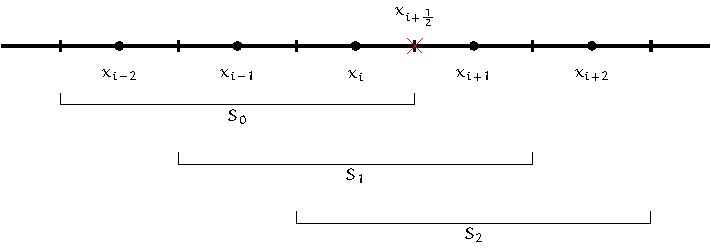
\includegraphics[width=\textwidth]{interpolation_stencils.pdf}
   \caption{Interpolation domain for $r=3$}
   \label{fig:stencils_3}
\end{figure}

\begin{equation}
  \label{eq:pol_0}
  p_0(x_{i+\frac{1}{2}}) = \frac{3}{8} u_{i-2} - \frac{5}{4} u_{i-1} + \frac{15}{8} u_i
\end{equation}

and this approximation is third order accurate if the function $u(x)$ is smooth in the stencil $S_0$. If we choose a different stencil $S_1=\left\{ x_{i-1}, x_{i}, x_{i+1} \right\}$ we obtain the polynomial $p_1$:

\begin{equation}
  \label{eq:pol_1}
  p_1(x_{i+\frac{1}{2}}) = -\frac{1}{8} u_{i-1} + \frac{3}{4} u_i + \frac{3}{8} u_{i+1}
\end{equation}

that is also third order accurate. The last stencil that can be used is the stencil $S_2=\left\{ x_{i}, x_{i+1}, x_{i+2} \right\}$ to obtain the third order accurate interpolating polynom $p_2$:

\begin{equation}
  \label{eq:pol_2}
  p_2(x_{i+\frac{1}{2}}) = \frac{3}{8} u_i + \frac{3}{4} u_{i+1} - \frac{1}{8} u_{i+2}
\end{equation}

Using \eqref{eq:Lagrange_big} on the stencil $S= S_0 \cup S_1 \cup S_2$, we obtain a fifth order accurate approximation of the function $u$ at the point $x_{i+\frac{1}{2}}$:

\begin{equation}
  \label{eq:pol_union}
  P(x_{i+\frac{1}{2}}) = \frac{3}{128} u_{i-2} - \frac{5}{32} u_{i-1} + \frac{45}{64} u_i + \frac{15}{32} u_{i+1} - \frac{5}{128} u_{i+2}
\end{equation}

Using~\ref{eq:pol_convex}, for this particular case by simple algebra the following values for linear weights can be obtained: $\gamma_0 = \frac{1}{16}$, $\gamma_1 = \frac{5}{8}$, $\gamma_2 = \frac{5}{16}$.

The smoothness indicators coefficients $\sigma_{k,j,l}$ can be obtained applying equation~\ref{eq:IS} to $p_0$, $p_1$ and $p_2$ polynoms respectively; this leds to the three explicit formulas for $\beta_k$:

\begin{align}
   \beta_0 & = \frac{ 4}{3} u_{i-2}^2 - \frac{19}{3} u_{i-2} u_{i-1} + \frac{25}{3} u_{i-1}^2 + \frac{11}{3} u_{i-2} u_{i  } -\frac{31}{3} u_{i-1} u_{i  } + \frac{10}{3} u_{i  }^2 \\
   \beta_1 & = \frac{ 4}{3} u_{i-1}^2 - \frac{13}{3} u_{i-1} u_{i  } + \frac{13}{3} u_{i  }^2 + \frac{ 5}{3} u_{i-1} u_{i+1} -\frac{13}{3} u_{i  } u_{i+1} + \frac{ 4}{3} u_{i+1}^2 \\
   \beta_2 & = \frac{10}{3} u_{i  }^2 - \frac{31}{3} u_{i  } u_{i+1} + \frac{25}{3} u_{i+1}^2 + \frac{11}{3} u_{i  } u_{i+2} -\frac{19}{3} u_{i+1} u_{i+2} + \frac{ 4}{3} u_{i+2}^2
\end{align}

These expressions are used in equation~\ref{eq:nonlinear_weights} or in equation~\ref{eq:weno_M} or in equation~\ref{eq:weno_Z} to obtain the non-linear weights that are used in equation~\ref{eq:WENO_interp}.

When the interpolation target point isn't located at the cell interfaces ($x_{i-\frac{1}{2}}$ or $x_{i-\frac{1}{2}}$), some of the linear weigths could become negative
